\chapter{Desenvolvimento}\label{cap_exemplos}

Este capítulo é parte principal da dissertação e deve conter a exposição ordenada e detalhada do assunto. 
Divide-se em seções e subseções, 
em conformidade com a abordagem do tema e do método, abrangendo: 
revisão bibliográfica, materiais e métodos, técnicas utilizadas, resultados obtidos e discussão.

O conteúdo deste documento visa apresentar um tutorial para utilização da classe PPGCCUFSJ, utilizando a estrutura de trabalhos acadêmicos, 
mas por questões didáticas adotou-se capítulo, seções e subseções diferentes das usualmente utilizadas.

\section{Classe PPGCCUFSJ e modelo de trabalho de acadêmico}

A classe PPGCCUFSJ é uma derivada de um antigo modelo utilizado no Instituto de Ciências Matemáticas e de Computação (ICMC) de São Carlos, Universidade de São Paulo (USP):

O objetivo do projeto é disponibilizar um modelo em \LaTeX\  para a elaboração de trabalhos acadêmicos (dissertação, trabalho de conclusão de curso (TCC), dentre outros) em conformidade com as normas do departamento de Ciência da Computação (DCOMP) da UFSJ. 

Este documento e seu código fonte são exemplos de uso da classe PPGCCUFSJ e do pacote \textsf{natbib}.

\section{Codificação dos arquivos: UTF8}

A codificação \texttt{UTF8} deve ser utilizada para todos os arquivos. 
Utilize a mesma codificação nos documentos que escrever, 
incluindo nos arquivos de base bibliográficas |.bib|. 
Para tanto, o arquivo \texttt{main.tex} deve conter o seguinte pacote:
\begin{verbatim}
\usepackage[utf8]{inputenc}	 
\end{verbatim}

\section{Tabelas}

As tabelas e os quadros apresentam os dados de modo resumido, 
oferecendo uma visão geral do conteúdo em questão, 
visando facilitar a compreensão do fenômeno em estudo. 
A diferença básica entre ambas está relacionada ao conteúdo e a formatação. 
Um exemplo de tabela é mostrado na página seguinte (Tabela~\ref{tab:descriptive_statistics_treatment}).\footnote{
A Tabela~\ref{tab:descriptive_statistics_treatment} foi extraída de \citet{please_please_me}.
}

\begin{table}[!htb]
	\caption{Sumário das características do grupo de tratamento~\citep{please_please_me}.\label{tab:descriptive_statistics_treatment}}
	\begin{center}
		\footnotesize
		\tabcolsep=0.11cm
		\begin{tabular}{ l | r | r | r | r |}
		 \cline{2-5}
		 &\multicolumn{4}{c|}{\textbf{Overview of the Treatment Group}} \\
		 \cline{2-5}
		 \multicolumn{1}{ l |}{\textbf{}} & \multicolumn{1}{c|}{\textbf{Google Play Reviews}} & \multicolumn{1}{c|}{\textbf{Rating}} & 
		 \multicolumn{1}{c|}{\textbf{Lifespan}} & \multicolumn{1}{c|}{\textbf{Commits}} \\
		\hline
		\multicolumn{1}{| r |}{\textbf{Max}} & 624,366 & 4.8 & 2,976 & 11,049 \\
		\hline
		\multicolumn{1}{| r |}{\textbf{Min}} & 91 & 3 & 759 & 31 \\
		\hline
		\multicolumn{1}{| r |}{\textbf{Mean}} & 31,658.4 & 4.27 & 1,873.80 & 2,704.53\\
		\hline
		\multicolumn{1}{| r |}{\textbf{Trimmed}} & 7,389.04 & 4.35 & 1,895.29 & 2,318.67 \\
		\hline
		\multicolumn{1}{| r |}{\textbf{Median}} & 3,523.0 & 4.4 & 2,113.5 & 1,682.5 \\
		\hline
		\multicolumn{1}{| r |}{\textbf{Std Dev}} & 113,831.38 & 0.42 & 641.29 & 2,748.98 \\
		\hline
		\multicolumn{1}{| r |}{\textbf{MAD$^\ddag$}} & 4,918.53 & 0.22 & 491.48 & 2,029.68 \\
		\hline
		\multicolumn{5}{| l |}{$^\ddag$MAD stands for median absolute deviation.} \\
		\hline
		\end{tabular}
	\end{center}
\end{table}

\section{Figuras} 

Figuras podem ser criadas diretamente em \LaTeX ou podem ser 
incorporadas por meio de um arquivo externo, 
como é o caso da Figura~\ref{fig:execution_flow}.\footnote{A Figura~\ref{fig:execution_flow} foi extraída de \citet{speeding_up_mutation_testing}.} 
É importante que sejam utilizadas imagens vetoriais no formato PDF. 
Com isso, o tamanho do arquivo final do trabalho será menor e as imagens terão uma apresentação melhor, 
principalmente quando impressas, uma vez que imagens vetoriais são perfeitamente escaláveis para qualquer dimensão. 

\begin{figure}[H]
 \center
 \scalebox{0.6}{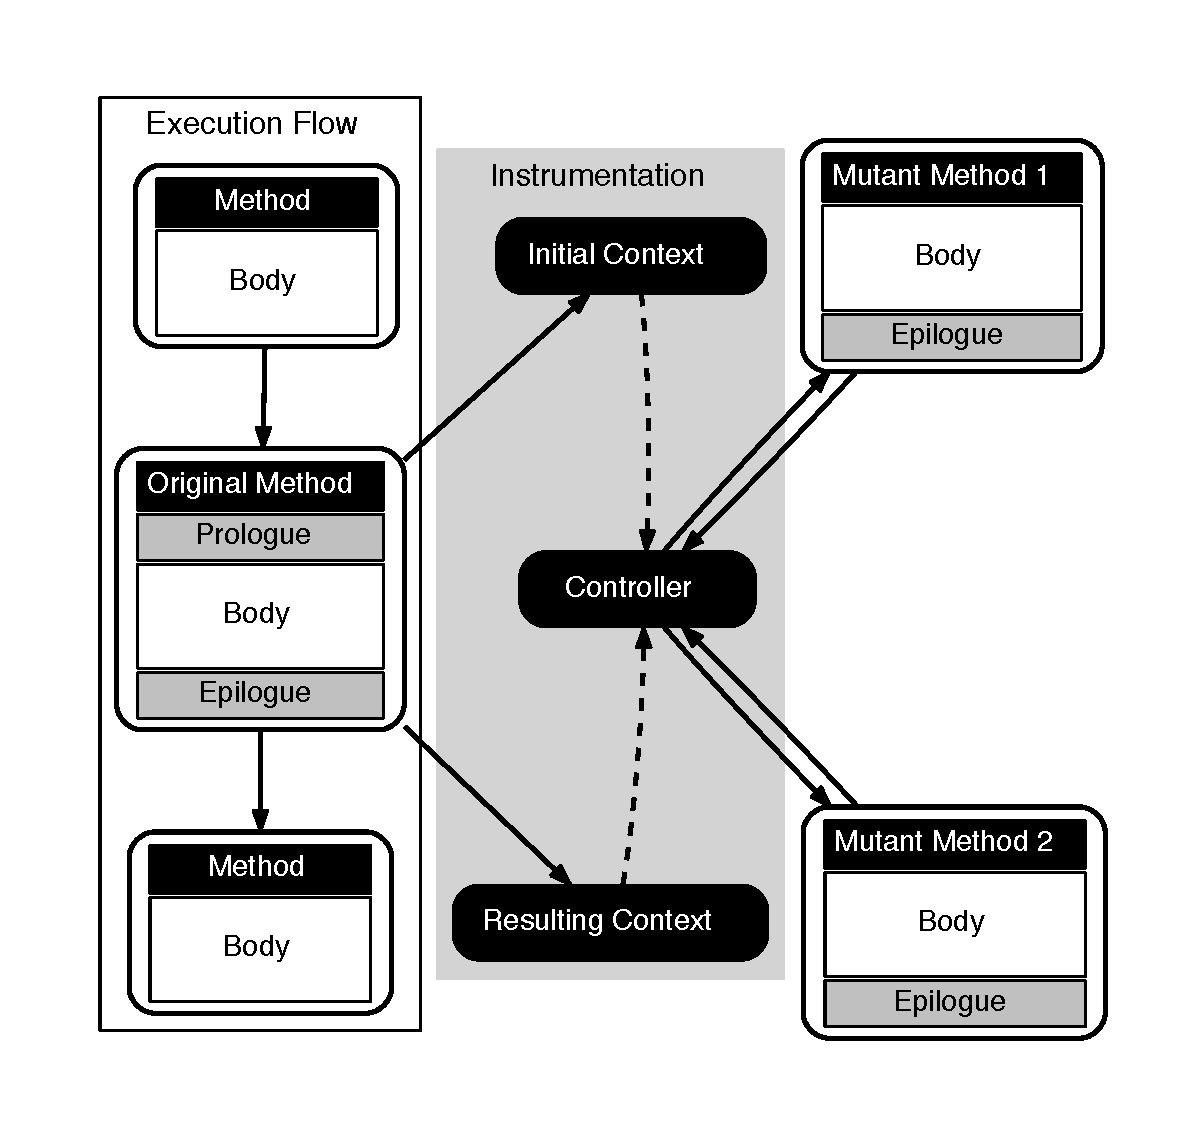
\includegraphics{execution_flow_overview}}
 \caption{Visão geral do pré-processamento de métodos originais antes de serem compilados pela máquina virtual Java.}
 \label{fig:execution_flow}
\end{figure}

\section{Diferentes idiomas e hifenizações}
\label{sec-hifenizacao}

Para usar hifenizações de diferentes idiomas, inclua nas opções do documento o
nome dos idiomas que o seu texto contém. Os usuários da classe PPGCCUFSJ devem utilizar:

\begin{verbatim}
\usepackage[english, %idioma adicional
portuguese]{babel} 
\end{verbatim}

Desta forma o texto deverá ser escrito idioma português-brasileiro (\texttt{brazil}), podendo ter citações em inglês.
Os idiomas português-brasileiro (\texttt{brazil}) e inglês são incluídos automaticamente pela classe.

